% HEADS UP: GIT IS NOT UP TO DATE

\documentclass[aps,rmp,reprint,amsmath,amssymb,graphicx,longbibliography]{revtex4-1}

\usepackage{bm}
\usepackage{graphicx}
\usepackage{epstopdf}
\usepackage{wrapfig}
\usepackage{array}
\usepackage{listings}
\usepackage[para,online,flushleft]{threeparttablex}
\usepackage{booktabs,dcolumn}
\usepackage{color}
\usepackage{comment}


\usepackage{textpos}
\usepackage{booktabs}
\usepackage{multirow,bigdelim}
\usepackage{float}

\usepackage{upgreek} % upalpha in Saxena2021 Reference

\usepackage[utf8]{inputenc}
\usepackage{hyperref}
\hypersetup{breaklinks=true,colorlinks=true,linkcolor=blue,citecolor=blue,filecolor=magenta,urlcolor=blue}

\usepackage[table]{xcolor}
%\newcommand{\contrib}[1]{\textcolor{red}{#1}}
%\newcommand{\comment}[1]{\textcolor{blue}{#1}}
%\newcommand{\WN}[1]{{\color{red} #1}}

\makeatletter
\def\@bibdataout@aps{%
\immediate\write\@bibdataout{%
@CONTROL{%
apsrev41Control%
\longbibliography@sw{%
    ,author="08",editor="1",pages="1",title="0",year="1"%
    }{%
    ,author="08",editor="1",pages="1",title="",year="1"%
    }%
  }%
}%
\if@filesw \immediate \write \@auxout {\string \citation {apsrev41Control}}\fi
}
\makeatother


%\usepackage[left]{lineno}
%\linenumbers



\begin{document}
\pagenumbering{gobble}

\title{Regression Analysis and Resampling Methods}

\author{Andreas Isene$^*$}
\author{Christian D. Nguyen$^*$}
\author{Daniel Fremming$^*$}

% TODO: Change and apply affiliation
% \affiliation{Department of Physics and Center for Computing in Science Education, University of Oslo, N-0316 Oslo, Norway}
% \affiliation{Department of Physics and Center for Computing in Science Education, University of Oslo, N-0316 Oslo, Norway}
% \affiliation{Department of Physics and Center for Computing in Science Education, University of Oslo, N-0316 Oslo, Norway}


% The abstract gives the reader a quick overview of what has been done and the most important results.
\begin{abstract}
     In this paper we use regression methods such as OLS, ridge and lasso regression to fit the two-dimentional franke's function. We explore bias-variance trade-off and compare bootstrapping with cross-validation to improve our model. The model is then applied to real terrain data.
\end{abstract}

\maketitle
\def\thefootnote{*}\footnotetext{These authors contributed equally to this work}\def\thefootnote{\arabic{footnote}}
\def\thefootnote{$^1$}\footnotetext{For full excerpt of conversion with chatGPT, see github material}

\tableofcontents


%Introduction should contain:

%Motivate the reader, the first part of the introduction gives always a motivation and tries to give the overarching ideas

%What I have done

%The structure of the report, how it is organized etc

%TODO: summary of work, structure of report
\section{Introduction}
Regression analysis is a central tool in science as a whole. It can be utilized to make predictions based on multiple independent variables. As an example one could predict house prices based on location, size, number of rooms, etc. There are various different methods that has been developed, each with unique strengths and weaknesses. As such we have been motivated to explore specifically \textit{ordinary least squares}, \textit{ridge regression}, and \textit{lasso regression}. These methods have been applied to fit models on real topographic data. They were then be evaluated and improved through resampling techniques. 

This is some simple reference \cite{Goodfellow2016}.
This is another elaborate reference \cite{Hastie,raschka2022}
In conversation with GPT we established that it liked ice cream $^1$.

\begin{comment}
    \section{Template: Artificial Intelligence and Machine Learning for nuclear physics in broad strokes}
    
    
     Statistics, data science, and AI/ML form important fields of research
     in modern science. They describe how to learn and make predictions
     from data, and enable the extraction of key information about
     physical processes and the underlying scientific laws based on large
     datasets. As such, recent advances in AI capabilities are being
     applied to advance scientific discoveries in the physical sciences.




Ideally, AI represents the science of building models to perform a
task without being explicitly programmed. ML tasks fall under the
broader AI umbrella. We will henceforth refer to the methods discussed
as ``AI/ML''. The idea is that there exist generic algorithms which
can be used to find patterns in a broad class of datasets without
having to write code specifically for each problem. The algorithm
builds its own logic based on the data. The attentive reader should
however always keep in mind that machines and algorithms are to a
large extent developed by humans. The choice of a specific AI/ML
algorithm is governed by the insights and knowledge about a specific
system.



There exist many AI/ML approaches; they are often split into two main
categories, supervised and unsupervised. In supervised learning, data
are labeled and one lets a specific ML algorithm learn and deduce
patterns in the datasets. This allows one to make predictions about
future events and/or data not included in the training set.  On the
other hand, unsupervised learning is a method for finding patterns and
relationship in datasets without any prior knowledge of the
system. Many researchers also operate with a third category, dubbed
reinforcement learning. This is a paradigm of learning inspired by
behavioral psychology, where actions are learned to maximize reward.
One may encounter reinforcement learning being accompanied by
supervised deep learning methods. Furthermore, what is often referred
to as semi-supervised learning, entails developing algorithms that aim
at learning from a dataset that includes both labeled and unlabeled
data.


Another way to categorize AI/ML tasks is to consider the desired output of a system. Some of the most common tasks are:
\makeatletter
\renewenvironment{description}%
               {\list{}{\leftmargin=10pt % <------- Adjust this length
                        \labelwidth\z@ \itemindent-\leftmargin
                        \let\makelabel\descriptionlabel}}%
               {\endlist}
\makeatother


\begin{description}
    \item[Classification] Outputs are divided into two or more classes. The goal is to produce a model that assigns inputs into one of these classes. An example is to identify digits based on pictures of hand-written numbers.
\item[Regression] Finding a functional relationship between an input dataset and a reference dataset. The goal is to construct a function that maps input data into continuous output values.
\item[Clustering] Data are divided into groups with certain common traits, without knowing the different groups beforehand. This AI/ML task falls  under the category of unsupervised learning.
\item[Generation] Building a model to generate data that are akin to a training dataset in both examples and distributions of examples. Most generative models are types of unsupervised learning.
\end{description}
In Table\,\ref{tab:acronyms} we list many of the methods encountered in this work, with their respective abbreviations.
\begin{table*}[!htb]
 \caption{Table of AI/ML with indication on the main type of learning (S: supervised,  U: unsupervised,  Semi-S: semi-supervised).
 }
    \label{tab:acronyms}
\begin{ruledtabular}
    \begin{tabular}{cll}
    Acronym & Method & Type of Learning \\ \hline
    AE & Autoencoders & U \\
    ANN     & Artificial Neural Networks & S  \\
  BED & Bayesian Experimental Design   & S \\
        BM & Boltzmann Machines & U \\
    BMA & Bayesian Model Averaging & S \\
    BMM & Bayesian Model Mixing & Semi-S \\
    BO & Bayesian Optimization & S \\
    BNN & Bayesian Neural Networks & S \\
%  CL & Clustering Methods & U \\ %MPK none found in text
    CNN & Convolutional Neural Networks & S \\
     EMB  & Ensemble Methods  and Boosting, including Decision Trees and Random Forests & S \\
  %  FFNN & Feed Forward Neural Network & S \\  %MPK changed in text
    GAN & Generative Adversarial Networks  & U \\
    GP & Gaussian Processes  & Semi-S \\
    KNN & $k$-nearest neighbors & U \\
    KR & Kernel Regression & S \\
    LR & Logistic Regression & S\\
    LSTM & Long short-term memory & S\\
%    MLP & Multilayer Perceptron & S\\ %MPK changed in text
    PCA & Principal Component Analysis \& Dimensionality Reduction & U \\
    REG    & Linear Regression  & S \\
    RL & Reinforcement Learning & Neither S nor U \\
    RNN & Recurrent Neural Networks & S \\
    SVM & Support Vector Machines & S \\
    VAE & Variational Auto Encoders & U
     \end{tabular}
 \end{ruledtabular}
\end{table*}


The methods we cover here have three central elements in common,
irrespective of whether we deal with supervised, unsupervised, or
semi-supervised learning. The first element is some dataset (which can
be subdivided into training, validation, and test data), the second
element is a model, which is normally a function of some parameters to
be determined by the chosen optimization process. The model reflects
our prior knowledge of the system (or lack thereof). As an example, if
we know that our data show a behavior similar to what would be
predicted by a polynomial, fitting the data to a polynomial of some
degree would determine our model.  The last element is a so-called
cost (or loss, error, penalty, or risk) function which allows us to
present an estimate on how good our model is in reproducing the data
it is supposed to train. This is the function which is optimized in
order to obtain the best prediction for the data under study. The
simplest cost function in a regression analysis (fitting a continuous
function to the data) is the so-called mean squared error function
while for a binary classification problem, the so-called cross entropy
is widely used, see, e.g., \cite{Hastie, Goodfellow2016} for
more details. We will henceforth refer to this element as the
assessment of a given method.



Traditionally, the field of AI/ML has had its main focus on
predictions and correlations.  In AI/ML and prediction-based tasks, we
are often interested in developing algorithms that are capable of
learning patterns from existing data in an automated fashion, and then
using these learned patterns to make predictions or assessments of new
data. In some cases, our primary concern is the quality of the
predictions or assessments, with perhaps less focus on the underlying
patterns (and probability distributions) that were learned in order to
make these predictions.  However, in many nuclear physics studies, we
are equally interested in being able to estimate errors and find
causations.  In this Colloquium, we emphasize the role of predictions
and correlations as well as error estimation and causations in
statistical learning and ML.  For general references on these topics
and discussions of frequentist and Bayesian methodologies, see, e.g.,
\cite{goodfellow2016}.

\newpage

%\section{Exercise 1: Expectation values for ordinary least squares expressions}
Assumptions:
\begin{enumerate}
    \item $\varepsilon \text{ is independent from } x \text{ which gives: }\mathbb{E}[\varepsilon]=0)$
    \item $y=f(x) + \varepsilon$ \text{. Here we will simplify f=f(x)}.
    \item $f(x) \text{ is a fixed, deterministic function of } x \text{, hence }\\ \mathbb{E}[f(x)]=f(x)$
\end{enumerate}
\hfill\break
\subsection{The mean-square error of our model can be written:}
%
%_____________________________________
%
\begin{align*}
    & \text{MSE} = \mathbb{E}[(y-\Tilde{y})^2]\\
    & = \mathbb{E}[y^2-2y\Tilde{y}+\Tilde{y}^2]\\
    & = \mathbb{E}[y^2]-2\mathbb{E}[y\Tilde{y}]+\mathbb{E}[\Tilde{y}^2]\\
\end{align*}
%
We look into each term:
\begin{equation}
\mathbb{E}[y^2]
\end{equation}
\begin{equation}
    \mathbb{E}[y\Tilde{y}]
\end{equation}
\begin{equation}
    \mathbb{E}[\Tilde{y}^2]
\end{equation}
%
%Term 1 ____________
From (1) we have:
 \begin{align*}
     & \mathbb{E}[y^2]=\mathbb{E}[(f+\varepsilon)^2]=\mathbb{E}[f^2+2f\varepsilon+\epsilon^2]\\
     & = \mathbb{E}[f^2]+\mathbb{E}[\varepsilon^2]\\
     & =  \mathbb{E}[f^2]+\sigma^2 = f^2+\sigma^2
 \end{align*}
%Term 2 _________________
From (2):
\begin{align*}
    & \mathbb{E}[y\Tilde{y}]=\mathbb{E}[y]\mathbb{E}[\Tilde{y}]
     = \mathbb{E}[f+\varepsilon]\mathbb{E}[\Tilde{y}]\\
    & =\mathbb{E}[f]\mathbb{E}[\Tilde{y}]=f\mathbb{E}[\Tilde{y}]
\end{align*}
%Term 3 _________________
We have:
\begin{align*}
    & Var[\Tilde{y}]=\mathbb{E}[(\Tilde{y}]-\mathbb{E}[\Tilde{y}])^2]\\
    & = \mathbb{E}[\Tilde{y}^2-2\Tilde{y}\mathbb{E}[\Tilde{y}]+(\mathbb{E}[\Tilde{y}])^2]\\
    & = \mathbb{E}[\Tilde{y}^2]-2\mathbb{E}[\Tilde{y}]\mathbb{E}[\Tilde{y}]+(\mathbb{E}[\Tilde{y}])^2\\
    & = \mathbb{E}[\Tilde{y}^2]-(\mathbb{E}[\Tilde{y}])^2\\
    & \implies \mathbb{E}[\Tilde{y}^2]= Var[\Tilde{y}]+(\mathbb{E}[\Tilde{y}])^2
\end{align*}
%
Put the terms together:
\begin{align*}
    & \mathbb{E}[y^2]-2\mathbb{E}[y\Tilde{y}]+\mathbb{E}[\Tilde{y}^2]\\
    & = f^2+\sigma^2-2f\mathbb{E}[\Tilde{y}]+(Var(\Tilde{y})+(\mathbb{E}[\Tilde{y}])^2)\\
    & = f^2-2f\mathbb{E}[\Tilde{y}]+(\mathbb{E}[\Tilde{y}])^2+Var(\Tilde{y})+\sigma^2\\
    & \implies \mathbb{E}[(f-\mathbb{E}[\Tilde{y}])^2]+Var(\Tilde{y})+\sigma^2
\end{align*}

First term in above expression can be approximated:
\begin{equation}
    \mathbb{E}[(f-\mathbb{E}[\Tilde{y}])^2] \simeq \frac{1}{n}\sum_{i}(y_i-\mathbb{E}[\Tilde{y}])^2 \text{ ,where } f_i\simeq y_i
\end{equation}

From (4) we have that MSE can be written:
\begin{equation}
    \mathbb{E}[(f-\mathbb{E}[\Tilde{y}])^2] \simeq \frac{1}{n}\sum_{i}(y_i-\mathbb{E}[\Tilde{y}])^2 = Bias[\Tilde{y}]
\end{equation}

Similarly, the variance can be expressed as:
\begin{align*}
    \mathbb{E}[(\Tilde{y}-\mathbb{E}[\Tilde{y}])^2]\simeq\frac{1}{n}\sum_{i}(\Tilde{y_i}-\mathbb{E}[\Tilde{y}])^2 = Var[\Tilde{y}]
\end{align*}
%___________________________________________
Setting in both the bias and variance terms into the equation we then obtain:

$MSE=Bias(\Tilde{y})+Var(\Tilde{y})+\sigma^2$

\subsection{Discussing the terms}
\hfill\break
The bias term represents the error caused by in-built assumptions in our used method. It consists of the average prediction over all data sets subtracted with the desired regression function.
The variance term describes the difference between solutions for the data sets and their average(variance of the model arounds its mean) \cite{bishop_2006_pattern}.

As for the sigma term, it represents the variance of the error, i.e. the noise of our method, where this quantity is expected to be irreducible. Since the sigma term is irreducible we will omit its interpretation in this section. The equation of minimum squared error(MSE) can be regarded as the expected loss when using our regression model, where we desire to minimize the error. This minimization can be dubbed the bias-variance trade-off, since it is about striking a balance between the bias and variance term. As for interpreting the terms(bias and variance), we will look into 2 scenarios as to how model complexity affects their behaviour.
Let $\Tilde{y}$ denote our model. The more complex it is, the better it is to go through the data points, hence we will acquire a lower bias. Respectively, the variance will be higher because the a higher model complexity makes the model "move" through more data points and it learns the noise of the training data. This flexibility in the model will lead run into the problem of overfitting our model, it works well on the training data we input, but it will run into problems once given new data it has never "seen", i.e. overfitting makes the model less able to generalize.

If the model $\title{y}$ is too rigid, it will output a high bias and low variance, and the model is not sufficient to fit the data points - we say it will underfit. Similarly to the case with a  complex model, it will result in a poor generalization.





%\hfill\break
%%
\section{Studying MSE values through analysis of Bias-variance}
%
% Set background color and other options for lstlisting

\hfill\break
The main code is obtained from: \url{https://compphysics.github.io/MachineLearning/doc/LectureNotes/_build/html/chapter3.html#the-bias-variance-tradeoff.}
\hfill\break
Modified code uses $y=sin(x)+log(x^2)$ as the one-dimensional function.


    \begin{lstlisting}[language=Python]
    import matplotlib.pyplot as plt
    import numpy as np
    from sklearn.linear_model import LinearRegression, Ridge, Lasso
    from sklearn.preprocessing import PolynomialFeatures
    from sklearn.model_selection import train_test_split
    from sklearn.pipeline import make_pipeline
    from sklearn.utils import resample

    np.random.seed(2018)

    n = 40
    n_boostraps = 100
    maxdegree = 14


    # Make data set.
    x = np.linspace(-3, 3, n).reshape(-1, 1)
    y = np.sin(x) + np.random.normal(0, 0.1, x.shape)
    error = np.zeros(maxdegree)
    bias = np.zeros(maxdegree)
    variance = np.zeros(maxdegree)
    polydegree = np.zeros(maxdegree)
    x_train, x_test, y_train, y_test = train_test_split(x, y, test_size=0.2)

    for degree in range(maxdegree):
        model = make_pipeline(
            PolynomialFeatures(degree=degree), LinearRegression(fit_intercept=False)
        )
        y_pred = np.empty((y_test.shape[0], n_boostraps))
        for i in range(n_boostraps):
            x_, y_ = resample(x_train, y_train)
            y_pred[:, i] = model.fit(x_, y_).predict(x_test).ravel()

        polydegree[degree] = degree
        error[degree] = np.mean(np.mean((y_test - y_pred) ** 2, axis=1, keepdims=True))
        bias[degree] = np.mean((y_test - np.mean(y_pred, axis=1, keepdims=True)) ** 2)
        variance[degree] = np.mean(np.var(y_pred, axis=1, keepdims=True))
        print("Polynomial degree:", degree)
        print("Error:", error[degree])
        print("Bias^2:", bias[degree])
        print("Var:", variance[degree])
        print(
            "{} >= {} + {} = {}".format(
                error[degree],
                bias[degree],
                variance[degree],
                bias[degree] + variance[degree],
            )
        )

    plt.plot(polydegree, error, label="Error")
    plt.plot(polydegree, bias, label="bias")
    plt.plot(polydegree, variance, label="Variance")
    plt.legend()
    plt.show()
    \end{lstlisting}
Results from the bias and variance trade-off as function of the model complexity can be seen in the table ~\ref{tab:ModelComplexMSE} below.
Here we set the number of data points to 40 and bootstrap to 100 iterations.
Blue rows highlights where the model complexity yields the lowest error:

\begin{table}
    \centering
    \begin{tabular}{c|c|c|c}
        \textbf{Order} & \textbf{Error} & \textbf{Bias\textsuperscript{2}} & \textbf{Variance}\\
        \text{0} & 3.222694  & 3.104592   & 0.118102\\
        \text{1} & 2.637989  & 2.492254   & 0.145734 \\
        \text{2} & 1.234957 & 1.095855    & 0.139102\\
        \text{3} & 1.142538 & 0.978143   & 0.164395\\
        \text{4} & 0.604439 & 0.475311  & 0.129127\\
        \text{5} & \cellcolor{blue!25}0.578585 & \cellcolor{blue!25}0.4131747   & \cellcolor{blue!25}0.165410\\
        \text{6} & \cellcolor{blue!25}0.370845 & \cellcolor{blue!25}0.214435   &  \cellcolor{blue!25}0.156410\\
        \text{7} & \cellcolor{blue!25}0.435129 & \cellcolor{blue!25}0.229928  & \cellcolor{blue!25}0.205200\\
        \text{8} & 0.739773 & 0.360638   & 0.379134\\
        \text{9} & 1.179098 & 0.368951   & 0.810147 \\
        \text{10} & 0.917037& 0.390615   & 0.526421 \\
        \text{11} & 7.420075 & 0.278572  & 7.141503  \\
        \text{12} & 9.530186 & 0.267499  & 9.262687  \\
        \text{13} & 16.252874 & 0.147212 & 16.105661 \\
    \end{tabular}
    \caption{Bias and variance trade-off as function of polynomial complexity.}
    \label{tab:ModelComplexMSE}
\end{table}

\begin{figure}
    \centering
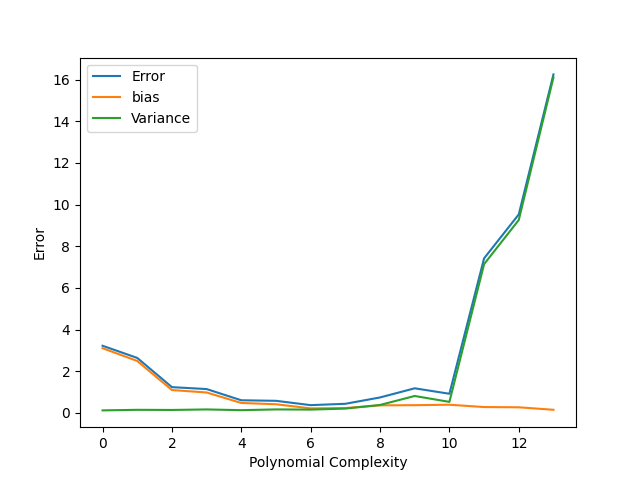
\includegraphics[width=1.0\linewidth]{figures/Figure_1.png}
    \caption{Plot Analysis of  plot of error, bias, and variance as function of increasing complexity}
    \label{fig:1}
\end{figure}

\newpage
\section{Bias-Variance Trade-Off}
%
\begin{itemize}
    \item \textbf{Low Complexity($<5$):} High bias and low error, the model underfits our test data and is not able to capture the complexity of our target function. This gives us a somewhat higher error.
    \item \textbf{Optimal Complexity($5-7$):} Our error is relatively low meaning that our model does a decent job in describing underlying patterns in the target function. This is provided by the bias-term. The variance on the other hand, is low enough so our model does not overfit. For the polynomial degree between 4-7 we can see that the trade-off between bias and variance is minimizes the error.
    \item \textbf{High Complexity($>7$):} The low bias describes now that our model is exceptional at fitting to our target function, but our model is now too specific - it is restricted to perform well with the data set we provided, but will struggle with new data sets. The high variance shows that our model has been overfitted and the higher error describes that our model is no longer suitable for generalization.
\end{itemize}
%
From the table we can see the error of the model is at its lowest when the degree of the polynomial is 6. This also holds true for visual inspection of the graph in figure ~\ref{fig:1}.

\section{Effect of Number of Data Points}

\hfill\break
From quick plots we observed that for low function complexity, the error, bias and variance stayed low (closer to $0$, seemingly). A major difference is the magnitude of error. On the y-axis we observed the error for (data points = 10) to take values between 0-700. When setting number of data points to 70, the error decreased and was within the range 0-3.5, but the error, bias and variance stayed at an all time low of zero until a polynomial degree of 10.

\section{Bootstrap Resampling}
As for bootstrap resampling we worked with the following number of bootstraps while holding number of samples fixed: (10,200).
For number of bootstraps= 10 the error varied where the bias was approximate close to the error to begin with. The graph of bias and errors stayed the same until degree 11 where error and variance were dominant and closer to each other and suddenly made a jump(see~\ref{fig:2}).
As for number bootstrap= 200, we had another behaviour. As depicted in figure~\ref{fig:3}.

\begin{figure}
    \centering
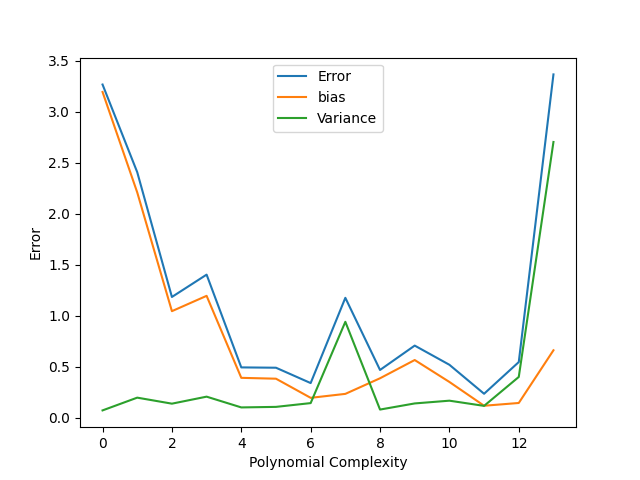
\includegraphics[width=1.0\linewidth]{figures/bootstrap 1.png}
    \caption{Plot Analysis of  plot of error, bias, and variance as function of increasing complexity}
    \label{fig:2}
\end{figure}

\begin{figure}
    \centering
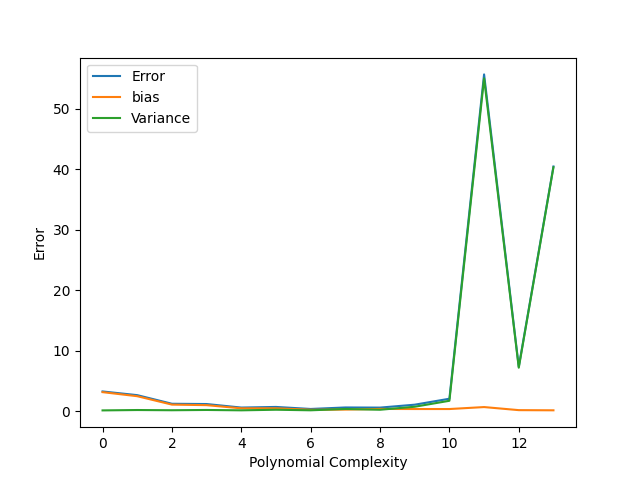
\includegraphics[width=1.0\linewidth]{figures/bootrstrap2.png}
    \caption{Plot Analysis of  plot of error, bias, and variance as function of increasing complexity}
    \label{fig:3}
\end{figure}



% Guidelines for references:
%Give always references to material you base your work on, either scientific articles/reports or books.
%Refer to articles as: name(s) of author(s), journal, volume (boldfaced), page and year in parenthesis.
%Refer to books as: name(s) of author(s), title of book, publisher, place and year, eventual page numbers
\end{comment}
\bibliographystyle{plain}
\bibliography{References} % add  references to this file
\end{document}
